\documentclass[10pt]{article}
% -------------------------------------------------------------------
% Pacotes básicos
\usepackage[english]{babel}
\usepackage[utf8]{inputenc}										
\usepackage[T1]{fontenc}
% -------------------------------------------------------------------
% Pacotes matemáticos
\usepackage{amsmath,amsfonts,amssymb,amsthm,cancel,siunitx,
calculator,calc,mathtools,empheq,latexsym}
% -------------------------------------------------------------------
% Pacotes de algoritmos e códigos
\usepackage{algpseudocode}
\usepackage{algorithm}
\usepackage{listings}
% -------------------------------------------------------------------
% Pacotes para inserção de figuras e subfiguras
\usepackage{subfig,epsfig,tikz,float}		            % Packages de figuras. 

\usepackage{blindtext}
\usepackage{hyperref}
% -------------------------------------------------------------------
% Pacotes para inserção de tabelas
\usepackage{booktabs,multicol,multirow,tabularx,array}          % Packages para tabela
\usepackage{natbib}
% -------------------------------------------------------------------
\setlength{\parindent}{0pt}
\setlength{\parskip}{5pt}
\textwidth 13.5cm
\textheight 19.5cm
\columnsep .5cm
% -------------------------------------------------------------------
% Título do seu artigo 
\title{\renewcommand{\baselinestretch}{1.17}\normalsize\bf%
\uppercase{Applied Mathematics Report: Finding Protein Conformations with Simulated Annealing in a 2D HP Lattice Model}
}
% -------------------------------------------------------------------
% Autorias
\author{%
Ellian Carlos Oliveira Costa$^{1*}$
}
% -------------------------------------------------------------------

%Início do documento

\begin{document}

\date{}

\maketitle

\vspace{-0.5cm}

\begin{center}
{\footnotesize 
*Corresponding author\\
$^1$ Universidade Federal Fluminense (first author) \\
E-mails: elliancarlos@gmail.com
}
\end{center}

% -------------------------------------------------------------------
% Abstract
\bigskip
\noindent
{\small{\bf ABSTRACT.}
Proteins are a vital part of any byological being, proteins dictacte uncountable mechanics in the human body and are a essencial part of life. Predicting the folding mechanism of a protein from its sequence of amino acids is the Protein Folding Problem (PFP). This report explores the application of Simulated Annealing (SA) to solve the Protein Folding Problem (PFP) within a 2D Hydrophobic-Polar (HP) Lattice Model.}

\medskip
\noindent
{\small{\bf Keywords}{:} Protein folding problem, H-P model; Minimal
energy conformation; 2D square lattice; Simulated
Annealing algorithm (SA).
}

\baselineskip=\normalbaselineskip
% -------------------------------------------------------------------

\section{Introduction}\label{sec:1}

Proteins are chains of polypeptides combined into a specific structure. Protein's structures plays a major role in its function and mechanics. The sequence of polypeptides is the primary structure of a protein and the final form of a single protein is called tertiary. A posible protein conformation that fits a fixed amino acid sequence is a fold. In nature, the process of folding a protein happens very fast and in such a way that minimizes the protein energy. The prediction of the minimal energy conformation of the protein given the sequence of amino acids is called the Protein Folding Problem (PFP).

Amino acids, which constitutes polypeptides, are either hydrophobic or hydrophilic, this single property can be used to caracterize the energy of the molecule for folding pourposes, as was  Lau and Dill's H-P Lattice Model \cite{DillAndLau1989}. This hydrophobic-hydropolar model is widely used for computationally solving the PFP. It is based on the fact that in their native state proteins minimize the internal energy in the folding process. This energy can be calculate counting the  uniques H-H contact in the lattice model, so the folding process maximizes the H-H contact. In this model, for every H-H contact a energy score of -1 is given. So it is posible to rewrite the PFP as finding the protein structure in a lattice square space such that the protein native fold $s*$ is the conformation that maximizes the energy function $E(s) = -1 \sum{\textit{\# of unique H-H contacts of s}}$ so: $s* = argmin\{E(s)/s \in S\}$, being $S$ the conformational space. The protein structure conformational space is every posiblity of a Self-Avoiding Walk in a 2D Lattice. This model simplifies the PFP problem, but it is still a very complex in both 2D lattices or 3D lattices, it's unfeasable to use exact methods since this problem is a NP-complete.

Solving the PFP in the HP Model has been a great area of reasearch, many lattice models, heuristics and meta heuritics have been developed and applied to the problem. In this report we focus to solve the problem with a simulated annealing in a HP 2D Square Lattice Model. 

The PFP problem is claimed to be resolved by AlphaFold in \cite{AlphaFold}, since 2021 the AlphaFold Protein Database has predicted over 200 million protein structure predictions from aminoacids sequence. Different from this work, they don't only predict the folding of the protein but its whole structure. AlphaFold is set to be the big thing for protein prediction since in a long time. 

\section{Code Disclaimer}

The model, the proposed algorithm and every computated resource was coded in Python 3.8 with the use of \verb|numpy| as the only external library, aside from \verb|numpy| and the native Python libraries all code was develop by the author. The code was done trying tried to adhere to good principles and POO techniques, at least as much as Python allows for its developers. All the code was run on a laptop with the 11th Gen Intel(R) Core(TM) i5-1135G7 CPU, 8GB of RAM in a NixOS Linux. If needed the author can provide more details about the configuration. Aside from the sent code, the code was also publicly available at \href{https://github.com/EllianCarlos/hp-lattice-model}{this repository} or at the url:\url{https://github.com/EllianCarlos/hp-lattice-model}.

\section{The HP Model Used}\label{sec:2}

The used HP Model is described in a 2D Lattice Space, and the protein structure is a Self Avoiding Walk in this 2D Lattice Space where every point is Polar (P) or Non-Polar (H), in this work this property will be called affinity. Be $s$ any solution for the protein structure in the conformational space, $s_i$ is the $i-th$ amino acid in the protein structure, affinity $a(s_i)$ of $s_i$ is:

$$
a(s_i) = \begin{cases}
      H & \text{if $s_i$ is hydrophobic.}\\
      P & \text{if $s_i$ is non-polar.}
    \end{cases}
$$

The 2D Square Lattice model is such that every point in the lattice has $4$ neighbors, one upwards, one downwards, one leftwards and one rightwards. A $s_i$ that is not the last nor the first amino acid in the sequence has a $s_{i-1}$ predecessor and a $s_{i+1}$ sucessor, a predecessor and a sucessor of a amino acid $s_i$, must be a neighbor of $s_i$. Every amino acid in the protein, must ocuppy one node in the lattice. A single node in the lattice can have either zero or one amino acid. This defines the constraints that build up the conformation space.

The energy of a conformation can be calculated via:

$$E(s) = -1 \cdot \sum_{i=1}^{n-2} \sum_{j=i+2}^{n} x_{ij} y_{ij} $$

$$
x_{ij} = \begin{cases}
     1 & \text{if $s_i = H$ and $s_j = H$  .}\\
     0 & \text{otherwise.}
    \end{cases}
$$

$$
y_{ij} = \begin{cases}
     1 & \text{if $s_i$ and $s_j$ contact each other .}\\
     0 & \text{otherwise.}
    \end{cases}
$$

For example, the following model has a energy of -2:



\subsection{Instances}

In this work we will cite the instances as a sequence of H and P characters representing each amino acid in the sequence and their affinity, for example: $PPHPHP$. Other used form of instance will be using chains o H and P characters alongside a expoent such that this number symbolize the number of times the last character or chain must be repeated, for example $P^2(HP)^2$ is the same as $PPHPHP$. 

All available and calculated instances in this report will be alongside the delivered code under the path $data/instances$, all of them in the $.dat$ extension which resolves only to a text string to the first representation in this section.

The test instances will be: 

\newcolumntype{C}{>{\centering\arraybackslash}X}
\begin{table}[!htb]
\centering
\begin{tabularx}{1.0\textwidth}{ c|c|C|c }
\toprule
I & L & Sequence & Native Energy \\ &&& $E(s*)$ \\ 
\midrule
0 & 6 & HP^2HPH & -2 \\
1 & 20 & (HP)^2PH(HP)^2(PH)^2HP(PH)^2 & -9 \\
2 & 24 & H^2P^2(HP^2)^6H^2 &  -9 \\
3 & 25 & P^2HP^2(H^2P^4)^3H^2 & -8 \\
4 & 40 & P^2H(P^2H^2)^2P^5H^{10}P^6(H^2P^2)^2HP^2H^5 &  -23 \\
\bottomrule
\end{tabularx}
\label{table:tab1}
\caption{Table of instances Is with their Length, Sequence and Energy.}
\end{table}

\subsection{Solutions}

All solutions will be saved locally automatically and describe in a text format with $.dat$ extension and will formated with the pattern: 

\begin{itemize}
    \item Each line contains only one piece of information
    \item Every file there is a separator that is a long sequence of the character -
    \item The lines until a separator are metadata, all lines after each describe the protein conformation
    \item Each line contains a KEY followed by a whitespace and then a VALUE
    \item In each line after the separator the KEY is the affinity of the amino acid and the VALUE the direction to append the aminoacid based on its predecessor
\end{itemize}

Example of a file with the solution of the first instance $I0$: 

\begin{lstlisting}
NAME 57ea5767-a0cc-4c8c-b345-80b1e6f740b2_model
ID: 57ea5767-a0cc-4c8c-b345-80b1e6f740b2
Energy: -2
---------------------------------
H None
P DOWN
P RIGHT
H UP
P UP
H LEFT
\end{lstlisting}

\subsection{Model Construction and Representation}

The HP Model was constructed in code with two major classes, one the \verb|Vertice| class representing a single amino acid in the HP model, this classes controls properties of each amino acid, as the polarity (hydrophobic or non-polar), pointers to others connected amino acids, distance to any other vertice and some static methods relative to utilities of vertices, like the movement of vertices. The other main class of the model is the \verb|Hp2dSquareModel|, which has all the utilities to control the chain of \verb|Vertices| or amino acids, it also has the utilities to load from a file and save the model to a file and calculate energy.

\begin{figure}
    \centering
    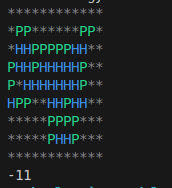
\includegraphics[width=0.35\linewidth]{example.png}
    \caption{Image of model's print with a print of the energy associated with it}
    \label{fig:enter-label}
\end{figure}

\section{The Algorithm}

The Simulated Annealing algorithm is among the most used meta-heuristics and it's based around a local search, it draws inspiration from the annealing termodynamics phenomena. The used version of SA is based on the paper \cite{SaInPFP}, it is called Improved Simulated Annealing, and the major differences are the neighbor function, which is constitute by a local move from a triangular lattice describe in \cite{LocalMoveSet} .

\begin{algorithm}
\caption{Simulated Annealing - SA($f(.), N(.), s, \alpha, SAmax, T_{0} $)}\label{alg:cap}
\begin{algorithmic}
% \textbf{Begin}
\Require The instance
\Ensure The best solution $s^*s$
\State $s \gets \text{ generate an initial solution in a random way};$
\State $s^* \gets \text{ the best solution } s;$
\State $T \gets \text{ initial temperatue };$
\State $T_{min} \gets \text{ minimal temperature };$
\State $k_{max} \gets \text{ maximum number of iteration after the use of diversification technique };$
\State $i \gets 0;$
\State $iterT \gets 0$
\While{$T \geq T_{min}$}
    \While{$iterT \geq SAmax$}
        \State $iterT \gets iterT + 1$
        \State $s' \gets \text{some } s \in \mathbf{N(s)}$
        \State $\Delta \gets f(s') - f(s)$
        \State $\delta \gets e^{\Delta / T}$ \Comment{$\delta \text{ is entropy}$}
        \If{$\Delta < 0 \text{ or } random~ u \in (0,1) < \delta$}
            \State $s \gets s'$
        \EndIf
        \If{$(f(s') < f(s^*))$}
            \State $s^* \gets s'$
        \Else
            \State $i \gets i + 1$
        \EndIf
        \If{$i = k_{max}$}
            \State $s \gets \text{some } s \in \mathbf{N(s)}$
            \State $i \gets 0$
        \EndIf
        \State $T \gets \alpha T$
    \EndWhile
\EndWhile
\end{algorithmic}
\end{algorithm}

\subsection{Algorithm Construction}

The algorithm construction was not an easy task as that was no previously publicated open source code from any of the authors of the base paper \cite{SaInPFP}. So the author had to build the HP Square Model by hand and also the so called Improved Simulated Annealing Algorithm. The SA algorithm bases itself on a neighbor function, that does a local search on a solution candidate. For every iteration on the algorithm a search $s' = N(s)$ is assigned, if $E(s') < E(s)$ a new solution $s$ is assigned, if $E(s') >= E(s)$, $s$ can be assigned to $s'$ if a random uniform generator generates a number is less than the actual entropy $e^{-\Delta / T}$. 

The parameters used were:

\newcolumntype{C}{>{\centering\arraybackslash}X}
\begin{table}[!htb]
\centering
\begin{tabularx}{1.0\textwidth}{ C | C }
\toprule
Parameter & Value \\ 
\midrule
$alpha$ & $0.90$ \\
$SA{_max} $ & $100$\\
$initial~temperature~T_0$ & $10000$\\
$K_{max}$ & $10$\\
\bottomrule
\end{tabularx}
\label{table:tab1}
\caption{Table of parameters.}
\end{table}

\subsection{The random generation of solutions}

The random generated solution is a basic Random Self Avoidance Walk (Random SAW) in the constructed model. There was tested a function \verb|generate_biased_random_solution| that generates a SAW that is sligthly biased to turn instead of continuing in the same path. This \verb|generate_biased_random_solution| did not generate any improvement in the model so it was not used after tests, but it was sended in the final code anyway.

\subsection{The Neighbor Function}

The neighbor function implemented was based on \cite{LocalMoveSet} where a vertice of the HP Square Model is diagonally move to improve H-H contacts and so improve connections. The author's implementation was done checking every move possible for every vertice in the model and evaluating its energy. The author tested two neighbor functions one that does the previous calculations and returns the best evaluated and other which returned any posible previous movement, even if it does not improves the model evaluation. The latter one was used, because it was left to the SA algorithm to the improvement instead of the neighbor and it was way faster than evaluating every movement posible.

The paper \cite{LocalRotation} was cited for a local rotation in the end of the SA algorithm, instead of another neighborhood search, but the author could not implement this feature in time, so the rotation isn't implemented in this report, but with more time, this would be posible and would probably improve results.

\section{Results}\label{sec:3}

The implemented algorithm was compared to other algorithms cited in this report, ISA for the Improved Simulated Annealing \cite{SaInPFP}, GA for the Genetic Algorithm \cite{GA} and ACO for the Ant Colony Optimization \cite{ACO}. The builded algorithm was run $100$ times for each of the instances and its results are in the column of Implemented ISA. 

\newcolumntype{C}{>{\centering\arraybackslash}X}
\begin{table}[!htb]
\centering
\begin{tabularx}{1.0\textwidth}{ C | C | C | C | C | C }
\toprule
Instance & Energy & ISA & GA & ACO & Implemented ISA \\ 
\midrule
0 & \textbf{-2} & No Data & No Data & No Data & \textbf{-2} \\ 
1 & \textbf{-9} & \textbf{-9} & \textbf{-9} & \textbf{-9} & -7 \\ 
2 & \textbf{-9} & \textbf{-9} & \textbf{-9} & \textbf{-9} & -7 \\ 
3 & \textbf{-8} & \textbf{-8} & \textbf{-8} & \textbf{-8} & -5 \\ 
4 & \textbf{-14} & \textbf{-14} & -12 & \textbf{-14} & -11 \\ 
\bottomrule
\end{tabularx}
\label{table:tab1}
\caption{Table of results to compare.}
\end{table}

As it occurs the implemented algorithm could not find the protein structure for any instance with enough complexity.

\section{Conclusions}\label{sec:4}

The implemented algorithm was able to optimize in some sort the model from random solutions, but it was heavily dependent on two things, one the neighbor function, as said before the author only implemented a local move set from \cite{LocalMoveSet}, but not the rotation from \cite{LocalRotation}, so the results was not able to rivalize with the algorithm from \cite{SaInPFP}, so this was a set back for the algorithm, another point was that the algorithm depends heavily on the random generated instance, as the classical SA  meta-heuristic it heavily depends on the first guess to do a good local search, and based on that search, improves the solution, far from optimal solutions even with search will still be far from optimal optimized solutions, so the algorithm depends on it.

The author firmly believes the algorithm was a success since it was able to optimize a HP 2D Square Lattice model to represent folding proteins, even though it did not rivalized with the current methods it was a great learning opportunity. The author also firmly bealives that upon improving the neighborhood search method and applying the given rotation in \cite{LocalRotation}, this algorithm can even best the current solutions.


\newpage

% FIM DO CONTEÚDO DO DOCUMENTO
% -----------------------------
\bibliographystyle{apalike} % Estilo de Bibliografia
\bibliography{referencias.bib} % Lista de Referências Bibliográficas

\end{document}